\section{Relateret produkter og undersøgelser}
\label{RelateretProdukterOgUndersoegelser}
%
I det følgende afsnit vil der være en kort gennemgang af produkter og undersøgelser, som i en eller anden grad relaterer sig til den sideløbende opgave, der blev præsenteret i foregående afsnit. Produkterne og undersøgelserne vedrører derfor enten interaktion med et interaktivt kunstværk, gestikker brugt til perifer interaktion med en musikafspiller eller perifer interaktion anvendt i andre sammenhænge. \blankline
%
Med udgangspunkt i konceptet omkring interaktion med et interaktivt kunstværk forekommer der flere elektroniske billedrammer på markedet. Blandt disse billedrammer er der særligt to, som skiller sig ud, da de interageres med via semaforiske gestikker; nemlig Meural, \parencite{WEB:Meural}, og Framed 2.0, \parencite{WEB:Framed2.0}. Både Meural og Framed 2.0 er bygget op omkring en platform, som tillader brugeren frit, at vælge hvad der skal præsenteres på det interaktive kunstværk. De to produkter tillader, at kunstnere fra over alt i verdenen har mulighed for at uploade og sælge deres kunst. Brugeren har derfor adgang til en database hvori et stort udvalg af kunstværker kan købes og tilføjes til forskellige afspilningslister. Derudover har brugeren også mulighed for selv, at uploade private billeder til diverse afspilningslister. Udover at både Meural, \parencite{WEB:Meural}, og Framed 2.0, \parencite{WEB:Framed2.0}, kan styres igennem en tilknyttet applikation, så kan de ligeledes styres via semaforiske gestikker, da begge produkter er udstyret med bevægelsessensorer. Brugeren har, ved de semaforiske gestikker, mulighed for, at skifte kunstværk ved at swipe enten fra højre mod venstre eller venstre mod højre. Derudover har Meural, \parencite{WEB:Meural}, en funktion, som tillader brugeren at få information omkring det specifikke kunstværk. Brugeren får adgang til denne information ved at hæve hånden foran kunstværket og for at fjerne informationsboksen sænkes hånden igen. 

Foregår interaktionen med de to produkter via de valgte semaforiske gestikker forudsættet det dog, at brugeren er tæt på billedrammen, for at bevægelsessensorne kan registrer bevægelsen. I relation til Bang $\&$ Olufsens ønske om, at interaktionen ikke skal være begrænset af afstanden til produktet, så kan der ikke drages en direkte parallel til hverken Meural, \parencite{WEB:Meural}, eller Framed 2.0, \parencite{WEB:Framed2.0}. Dog kan der drages paralleller til interaktionsformen; brugen af de semaforiske gestikker.\blankline
%
Udover produkter, der er sammenlignelige med Bang $\&$ Olufsens koncept om et interaktivt kunstværk, som portrætterer brugerens albumsamling og som tillader brugeren, at kontrollere musikken perifert, så er der foretaget nogle få undersøgelser, som netop vedrører perifer interaktion med en musikafspiller. 

En af de undersøgelser er foretaget af \textcite{PDF:ComparingInputModalities}, som har undersøgt om tre forskellige modaliteter, hvoraf to er manipulerende gestikker og én er semaforisk, kan understøtte perifer interaktion med en musikafspiller, når brugeren sidder foran sin computer. Først blev det undersøgt hvilke manipulerende og semaforiske gestikker, der skulle bruges til de mest basale funktioner en musikafspiller indeholder; start, pause, skift nummer frem eller tilbage og skrue op eller ned for lyden, \parencite[s. 165]{PDF:ComparingInputModalities}. De to manipulerende gestikker udføres enten via et knop-baseret håndtag eller en touchskærm, hvor den semaforiske gestik udføres over en plade, \parencite[s. 166]{PDF:ComparingInputModalities}. De tre modaliteter er repræsenteret på \autoref{fig:InputModalitiesMusicControl}
%
\begin{figure}[H]
	\centering
	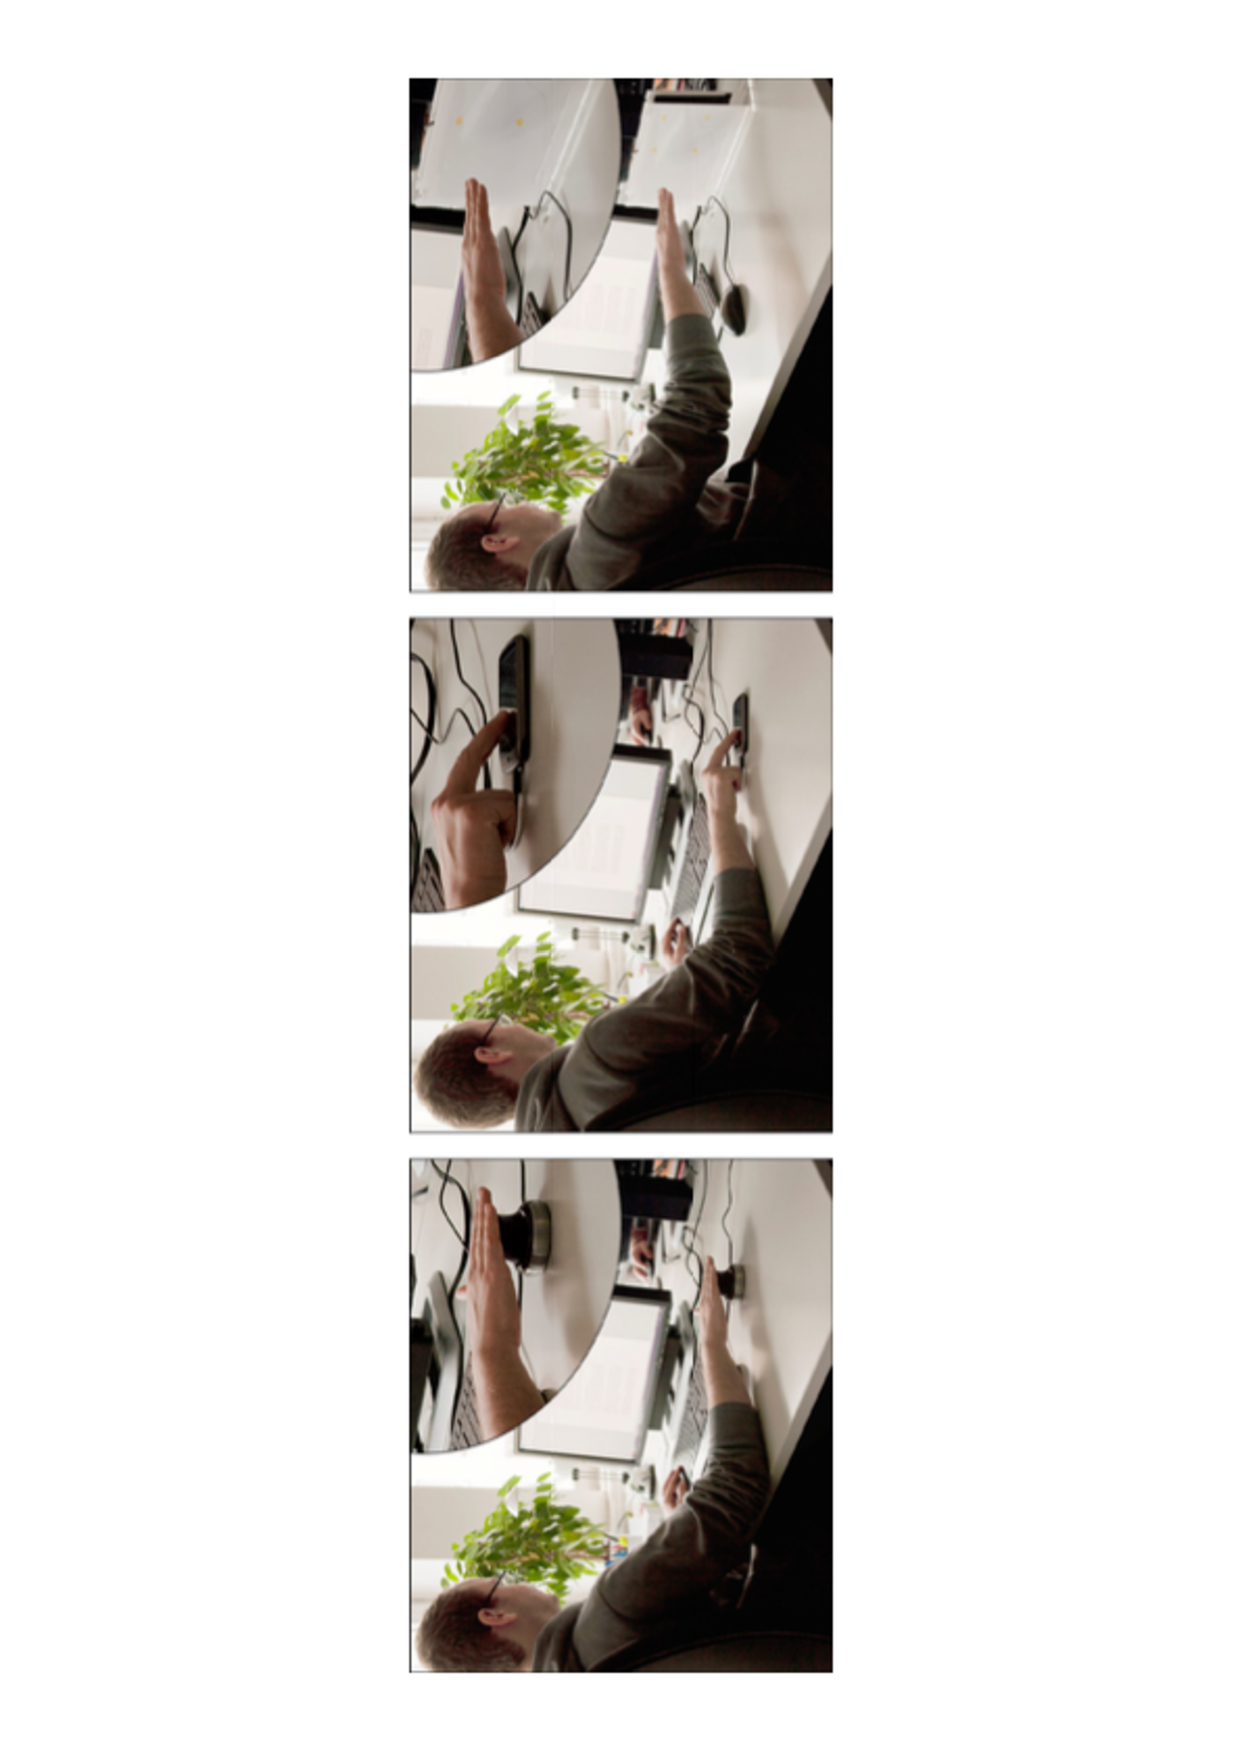
\includegraphics[resolution=300,width=0.70\textwidth, angle=-90]{InputModalitiesMusicControl}
	\caption{Illustration af de tre modaliteter, der bruges til perifer interaktion, fra venstre mod højre; knop-baseret håndtag, touchskærm og semaforisk gestik, \parencite[s. 163]{PDF:ComparingInputModalities}.}
	\label{fig:InputModalitiesMusicControl}
\end{figure}
\noindent
%
Herefter foretog \textcite[ss. 169-174]{PDF:ComparingInputModalities} en otte ugers feltundersøgelse, hvor testpersonerne skulle bruge hver af de tre modaliteter igennem en to ugers periode samt tastaturets egne funktioner. For at undersøge om det var muligt, at allokere interaktionen med musikafspilleren til det perifere, målte \textcite[ss. 172-173]{PDF:ComparingInputModalities}, hvor mange gange testpersonerne var i stand til at interagere med musikafspilleren, iTunes, uden at denne var i fokus. Deraf fremgår det, baseret på testpersonernes bemærkninger, at de i højere grad var i stand til at udføre interaktionen, uden at rette fokus mod iTunes, ved det knop-baseret håndtag og dernæst touchskærmen, \parencite[ss. 172]{PDF:ComparingInputModalities}. Testpersonerne rangerede de semaforiske gestikker sidst, da de, ifølge \textcite[ss. 172-173]{PDF:ComparingInputModalities}, dels manglede den haptiske feedback og dels nød at overvære ændringerne i iTunes forårsaget af deres gestik, som føltes magiske. Sandsynligheden for at en interaktion opstod var størst ved de semaforiske gestikker, hvilket \textcite[s. 171]{PDF:ComparingInputModalities} pointerer kan skyldes registrerings problemer, dernæst touchskærmen efterfulgt af det knop-baseret håndtag og den mindst sandsynlige interaktion var tastaturet. Derudover resulterede interaktionen med de tre modaliteter, i den perifere opmærksomhed, i en lavere mentalbelastning sammenlignet med tastaturet, \parencite[s. 172]{PDF:ComparingInputModalities}. Denne forskel i mentalbelastning kan være med til at fremme antallet af interaktioner, da testpersonerne generelt interagerede oftere med de tre modaliteter fremfor tastaturet, hvilket kan skyldes at tastaturet forårsagede en større mentalbelastning, \parencite[ss. 174-175]{PDF:ComparingInputModalities}.    

Ifølge \textcite[ss. 173-174]{PDF:ComparingInputModalities}, så finder testpersonerne den nye interaktionsform, perifer interaktion, som værende et positivt tiltag, særligt fordi de kan kontrollere iTunes, uden at fjerne fokus fra den primære opgave. Endvidere forbinder testpersonerne de semaforiske gestikker futuristisk og sjovt, \parencite[s. 174]{PDF:ComparingInputModalities}. I relation til de semaforiske gestikker kommenterer \textcite[s. 177]{PDF:ComparingInputModalities}, at de egner sig til perifer interaktion og de formegentlig i højere grad vil være at foretrække, såfremt de implementeres korrekt.\blankline
%                    
I undersøgelsen foretaget af \textcite{PDF:AStudyOnTheUseOfSemaphoricGestures} fokuseres der ligeledes på hvordan en musikafspiller kan kontrolleres perifert, og specifik hvordan det kan lade sig gøre via semaforiske gestikker. På baggrund af denne undersøgelse fremgår det, at testpersonerne foretrækker at interaktionen bygger på semaforiske gestikker fremfor at interaktionen skal foregå via tastaturet, det gør sig særligt gældende når tastaturet var uden for rækkevidde ved den primære opgave, \parencite[s. 1963]{PDF:AStudyOnTheUseOfSemaphoricGestures}. Dog påpeger testpersonerne, at de oplevede udmattelse ved gentagne gange at skulle udføre de semaforiske gestikker, \parencite[s. 1963]{PDF:AStudyOnTheUseOfSemaphoricGestures}. Ifølge \textcite[s. 1963]{PDF:AStudyOnTheUseOfSemaphoricGestures} vil det ikke nødvendigvis være tilfældet i den korrekte kontekst, da der højst sandsynligt ikke vil forekomme lige så mange interaktioner sammenlignet med det specifikke testscenarie. \textcite[s. 1964]{PDF:AStudyOnTheUseOfSemaphoricGestures} konkluderer, at der er signifikante fordele ved at anvende semaforiske gestikker, som interaktionsform ved sekundære opgaver, og at restitutionstiden mellem udførelse af en sekundær opgave og den primære opgave mindskes sammenlignet med hvis interaktionen foregik via tastaturet.\blankline
%

Kigges der videre på perifer styring af musik, når brugeren sidder ved computeren, har \textcite[ss. 5-9]{PDF:AChairAsUbiquitousInputDevice} undersøgt, hvordan en fleksibel stol kan bruges til at styre musik i den perifere del af opmærksomheden. Undersøgelsen viser, at det, ved brug af en fleksibel stol, er muligt at styre musikken uden at forstyrre en primær opgave, men også at restitutionstiden var signifikant kortere ved brug af stolen end keyboardet eller en touchflade, \parencite[s. 7]{PDF:AChairAsUbiquitousInputDevice}. Brugeroplevelsen var generelt tilfredsstillende, da stolen var nem at lære og nem at bruge. Ifølge \textcite[s. 8]{PDF:AChairAsUbiquitousInputDevice} er en fleksibel stol altså en anden måde at udvidde designområdet for perifer interaktion, selvom der kan forekomme konflikter, hvis almindelige bevægelser bliver fortolket som kommandoer eller bevælgelserne på stolen ikke er socialt acceptable.

Alternativt til styring af musik har \textcite[s. 1]{PDF:FacilitatingPIDesignAndEvaluation} undersøgt, hvordan interaktion kan finde sted i den perifere del af opmærksomheden, når interaktionen består af lysstyrkejustering på en lampe ved brug af en pointer, der skal tiltes op og ned. Undersøgen viste, at forsøgspersoner godt kunne interagere med både en opmærksomhedskrævende opgave og lampen på samme tid, uden at nogen af opgaverne blev tilsideset, \parencite[ss. 20-21]{PDF:FacilitatingPIDesignAndEvaluation}. Dog blev ydeevnen nedsat ved begge opgaver i forhold til at udføre begge opgaver hver for sig. Det viste sig at det meste af den visuelle opmærksomhed rettede sig mod den opmærksomhedskrævende opgave, hvilket kan indikere, at lysjusteringen blev gjort i den perifere del af opmærksomheden. I forbindelse med perifer interaktion blev det også undersøgt hvilken feedback fra produktet brugeren har brug for, for at udføre den perifere opgave bedst muligt. Undersøgelsen viste, at ved udførelse af en opmærksomhedskrævende opgave samtidig med lysjusteringsopgaven, gav det de bedste resultater, når forsøgsersonen fik feedback fra flere modaliteter.  Undersøgelsen testede også, hvor godt opgaven med at justere på lyset perifert blev udført sammenlignet med at drikke vand, som i forvejen er en nem perifer opgave, \parencite[s. 20]{PDF:FacilitatingPIDesignAndEvaluation}. Her viste det sig, at selvom lysjusteringen gøres perifert, så forstyrrede det den primære opgave mere, end når der blev drukket vand som sekundær opgave. Dette bliver dog forklaret med, at forsøgspersonerne ikke har haft så meget tid til at lære at styre lampen, som de har haft til at lære at drikke vand. 

Vendes fokus igen mod Bang $\&$ Olufsen ses det altså fra andre produkter og studier, at idéen om at kunne styre et interaktivt kunstværk perifert og ved brug af gestikker virker mulig. Dog er det vigtigt at bemærke, at de relaterede produkter og undersøgelser, der er blevet gennemgået, ikke nødvendigvis gengiver hvad Bang $\&$ Olfensen ønsker at udvikle. Gestikker, der er blevet brugt til musikstyring ved computeren, kan derfor ikke med sikkerhed overføres direkte til styring af et interaktivt kunstværk, men kan derimod give et peg om hvilken retning undersøgelsen af gestikker skal bevæge sig i. Der er som beskrevet flere typer af gestikker, der kan bruges til at interagere i den perifere del af opmærksomheden og forskellige holdninger til, hvornår og hvorvidt feedback er nødvendigt. For at foretage præcise undersøgelser, der kan give en idé om, hvordan perifer interaktion med Bang $\&$ Olufensens produkt kan udføres er det nødvendigt at afgrænse til en mere konkret problemformulering.
